\documentclass[aspectratio=169,11pt]{beamer}
\usepackage[T1]{fontenc}
\usepackage{lmodern,amsmath,amssymb,mathtools,bm,booktabs,array,graphicx,tikz}
\usetikzlibrary{arrows.meta,positioning,calc,decorations.pathreplacing,patterns}
\definecolor{ink}{HTML}{17344D}\definecolor{accent}{HTML}{087E8B}\definecolor{pale}{HTML}{EDF5F5}\definecolor{gold}{HTML}{AD6B19}
\providecommand{\dd}{\,\mathrm{d}}\providecommand{\R}{\mathbb{R}}
\providecommand{\E}{\mathbb{E}}\providecommand{\Var}{\operatorname{Var}}
\providecommand{\Cov}{\operatorname{Cov}}\providecommand{\diag}{\operatorname{diag}}
\providecommand{\norm}[1]{\left\lVert#1\right\rVert}
\providecommand{\abs}[1]{\left|#1\right|}
\usefonttheme{professionalfonts}
\setbeamercolor{normal text}{fg=black,bg=white}
\setbeamercolor{frametitle}{fg=ink,bg=white}
\setbeamercolor{title}{fg=ink}\setbeamercolor{structure}{fg=accent}
\setbeamercolor{block title}{fg=ink,bg=pale}\setbeamercolor{block body}{fg=black,bg=pale!40}
\setbeamercolor{alerted text}{fg=accent}
\setbeamerfont{frametitle}{size=\Large,series=\bfseries}
\setbeamerfont{title}{size=\LARGE,series=\bfseries}
\setbeamertemplate{navigation symbols}{}
\setbeamersize{text margin left=.7cm,text margin right=.7cm}
\setbeamertemplate{frametitle}{\vspace{.18cm}\insertframetitle\par\vspace{.1cm}{\color{accent}\hrule height .6pt}\vspace{.12cm}}
\newcommand{\notestarget}{notes.pdf}\newcommand{\noteslabel}{Notes}
\setbeamertemplate{footline}{\hspace{.7cm}\color{ink}\scriptsize Mathematical Cardiology\quad\href{\notestarget}{\noteslabel}\hfill\insertframenumber\,/\,\inserttotalframenumber\hspace{.7cm}\vspace{.18cm}}
\setbeamercovered{invisible}
\hypersetup{pdfauthor={Zan Ahmad},pdftitle={Muscle force and the pressure--volume cycle},pdfpagemode=UseNone}
\begin{document}
\begin{frame}[plain]\vfill
{\small\color{accent} Mathematical Cardiology \quad Lecture 3}\par\medskip
{\raggedright\hyphenpenalty=10000\exhyphenpenalty=10000\LARGE\bfseries\color{ink} Muscle force and the pressure--volume cycle}\par\bigskip
Zan Ahmad\par\smallskip
{\small Fall 2023}\par\vfill\end{frame}
\renewcommand{\notestarget}{notes.pdf\#note-from-crossbridges-to-a-macroscopic-force}
\begin{frame}[t,fragile,label=slide-two-levels-of-a-pumping-system]{Two levels of a pumping system}
Crossbridges contribute force to muscle.\pause{}\par The ventricular wall turns tissue forces into chamber pressure.\pause{}\par A pressure--volume loop records chamber work, not individual crossbridge motion.
\end{frame}
\renewcommand{\notestarget}{notes.pdf\#note-from-crossbridges-to-a-macroscopic-force}
\begin{frame}[t,fragile,label=slide-add-forces-across-a-population]{Add forces across a population}
\[F=N\sum_j a_jf_j,\qquad a_j\ge0,\quad\sum_j a_j\le1.\]\pause{} The attached fraction and each attached bridge's state both affect total force.
\end{frame}
\renewcommand{\notestarget}{notes.pdf\#note-normalize-the-force-velocity-relation}
\begin{frame}[t,fragile,label=slide-a-load-speed-family]{A load--speed family}
\[v=b\frac{F_0-F}{F+a},\qquad a,b>0.\]\pause{} At $F=0$, $v_{\max}=bF_0/a$.\pause{}\par At $F=F_0$, $v=0$.
\end{frame}
\renewcommand{\notestarget}{notes.pdf\#note-normalize-the-force-velocity-relation}
\begin{frame}[t,fragile,label=slide-make-the-variables-dimensionless]{Make the variables dimensionless}
\[f=F/F_0,\quad u=v/v_{\max},\quad\alpha=a/F_0.\]\pause{}\[u=\frac{\alpha(1-f)}{f+\alpha}.\]\pause{} For $\alpha=1/3$, $u=(1-f)/(1+3f)$.
\end{frame}
\renewcommand{\notestarget}{notes.pdf\#note-normalize-the-force-velocity-relation}
\begin{frame}[label=slide-force-speed-and-power-figure]{Force, speed, and power}
\centering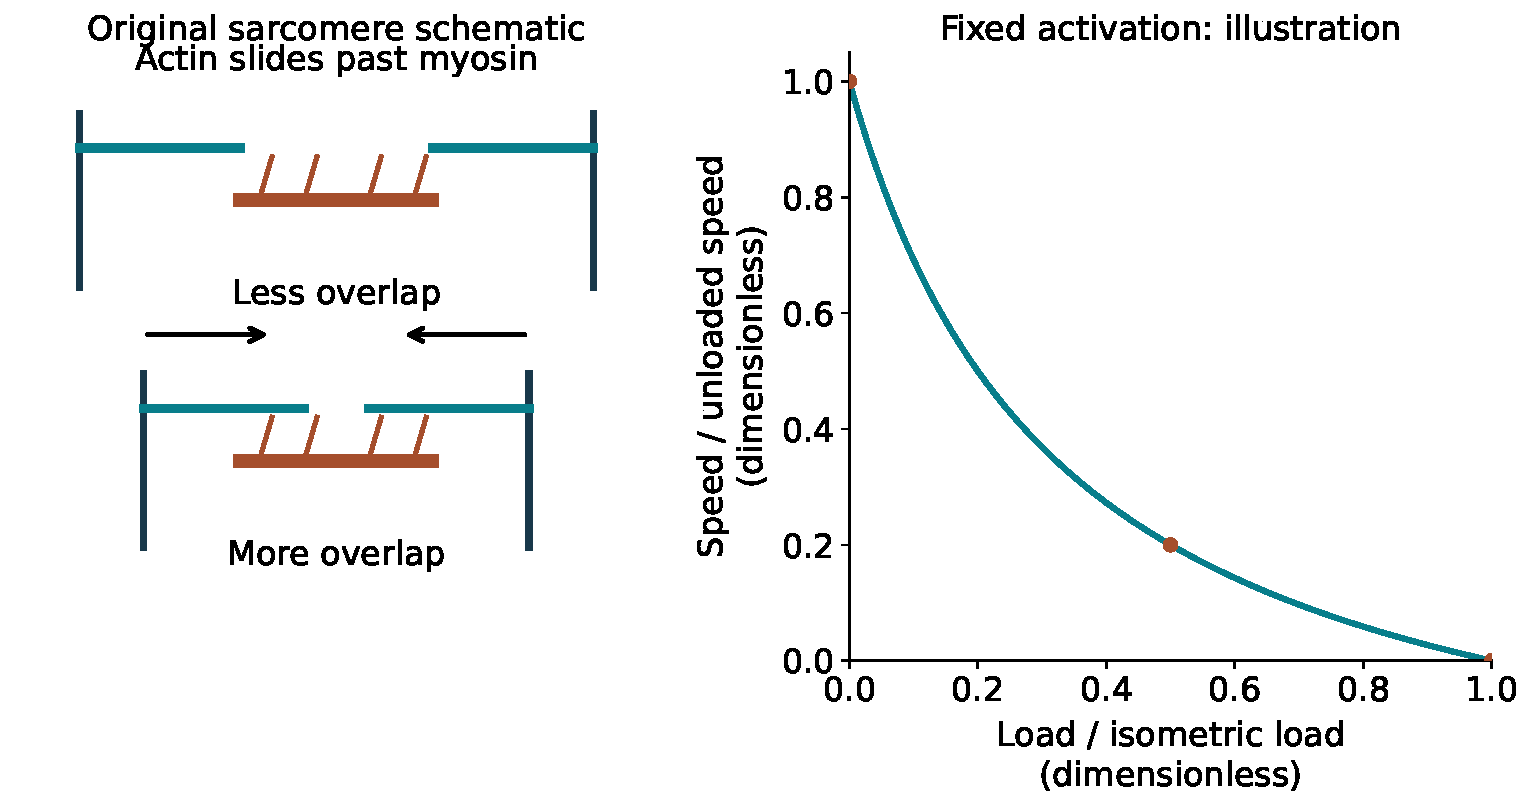
\includegraphics[width=.98\linewidth,height=.69\textheight,keepaspectratio]{muscle-and-load.pdf}\end{frame}
\renewcommand{\notestarget}{notes.pdf\#note-normalize-the-force-velocity-relation}
\begin{frame}[t,fragile,label=slide-force-speed-and-power]{Force, speed, and power}
\[f=\tfrac12\Rightarrow u=\frac{1/2}{5/2}=\tfrac15.\]\pause{}\[\text{normalized external power}=fu=\tfrac1{10}.\]\pause{} Zero shortening does not imply zero force or zero biochemical cost.
\end{frame}
\renewcommand{\notestarget}{notes.pdf\#note-a-loop-records-two-state-variables}
\begin{frame}[label=slide-the-pv-plane-figure]{The PV plane}
\centering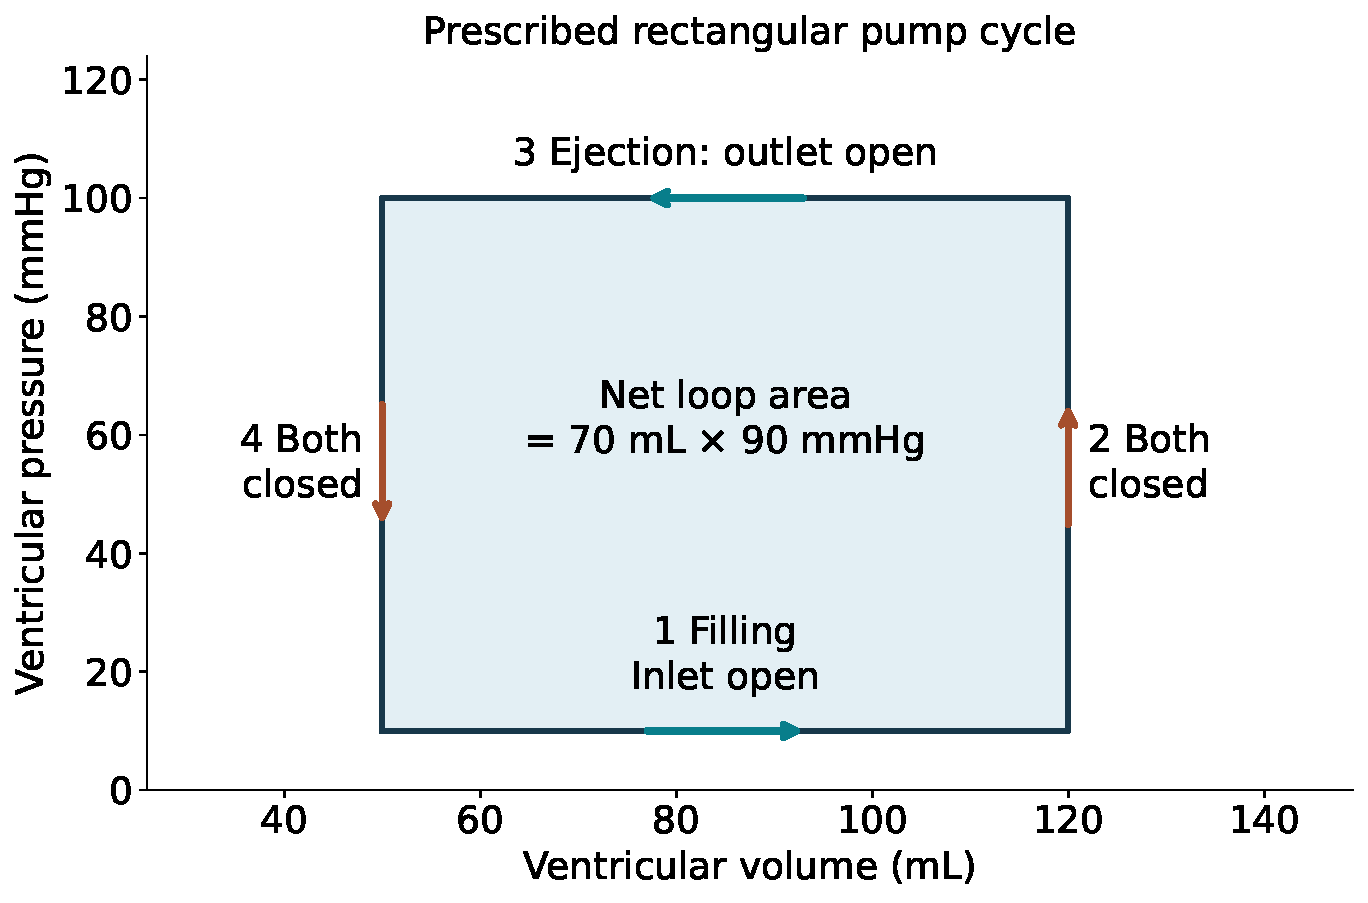
\includegraphics[width=.98\linewidth,height=.69\textheight,keepaspectratio]{pump-cycle.pdf}\end{frame}
\renewcommand{\notestarget}{notes.pdf\#note-a-loop-records-two-state-variables}
\begin{frame}[t,fragile,label=slide-the-pv-plane]{The PV plane}
Each point is $(V,P)$ at one instant.\pause{}\par A directed path shows the order of states.\pause{}\par Distance along the path does not specify the duration of a phase.
\end{frame}
\renewcommand{\notestarget}{notes.pdf\#note-a-loop-records-two-state-variables}
\begin{frame}[t,fragile,label=slide-filling]{Filling}
\[V:50\longrightarrow120\ \mathrm{mL},\qquad P=10\ \mathrm{mmHg}.\]\pause{} Mitral valve open; aortic valve closed in the idealized cycle.
\end{frame}
\renewcommand{\notestarget}{notes.pdf\#note-a-loop-records-two-state-variables}
\begin{frame}[t,fragile,label=slide-isovolumic-contraction]{Isovolumic contraction}
\[V=120\ \mathrm{mL},\qquad P:10\longrightarrow100\ \mathrm{mmHg}.\]\pause{} Both valves closed.\pause{}\par Fixed chamber volume does not mean inactive muscle.
\end{frame}
\renewcommand{\notestarget}{notes.pdf\#note-a-loop-records-two-state-variables}
\begin{frame}[t,fragile,label=slide-ejection-and-relaxation]{Ejection and relaxation}
At high pressure, volume falls from $120$ to $50$ mL.\pause{}\par Then both valves close and pressure falls at fixed volume.\pause{}\par The cycle returns to its starting state.
\end{frame}
\renewcommand{\notestarget}{notes.pdf\#note-stroke-volume-ejection-fraction-and-output}
\begin{frame}[t,fragile,label=slide-the-ejected-volume]{The ejected volume}
\[SV=EDV-ESV=120-50=70\ \mathrm{mL/beat}.\]\pause{} The retained $50$ mL is part of the next cycle's starting inventory.
\end{frame}
\renewcommand{\notestarget}{notes.pdf\#note-stroke-volume-ejection-fraction-and-output}
\begin{frame}[t,fragile,label=slide-a-fraction-is-not-an-efficiency]{A fraction is not an efficiency}
\[EF=\frac{SV}{EDV}=1-\frac{ESV}{EDV}=\frac{70}{120}.\]\pause{} Scale both chamber volumes by two: $EF$ stays fixed, while $SV$ doubles.
\end{frame}
\renewcommand{\notestarget}{notes.pdf\#note-stroke-volume-ejection-fraction-and-output}
\begin{frame}[t,fragile,label=slide-per-beat-to-per-minute]{Per beat to per minute}
\[CO=(70\ \mathrm{mL/beat})(75\ \mathrm{beats/min})\]\pause{}\[=5250\ \mathrm{mL/min}=5.25\ \mathrm{L/min}.\]\pause{} The calculation assumes identical repeated beats.
\end{frame}
\renewcommand{\notestarget}{notes.pdf\#note-derive-work-from-displaced-volume}
\begin{frame}[t,fragile,label=slide-why-pressure-times-volume-is-work]{Why pressure times volume is work}
\[\text{work}=(\text{force})(\text{distance})=(PA)\Delta x.\]\pause{}\[A\Delta x=\Delta V_{\rm displaced}.\]\pause{} Hence work is $P\Delta V_{\rm displaced}$.
\end{frame}
\renewcommand{\notestarget}{notes.pdf\#note-derive-work-from-displaced-volume}
\begin{frame}[t,fragile,label=slide-the-sign-of-chamber-work]{The sign of chamber work}
During ejection, chamber $\Delta V<0$.\pause{}\[W_{\rm delivered}\approx-P\Delta V.\]\pause{} Ejection contributes positively; filling contributes negatively under this convention.
\end{frame}
\renewcommand{\notestarget}{notes.pdf\#note-derive-work-from-displaced-volume}
\begin{frame}[t,fragile,label=slide-work-around-the-rectangle]{Work around the rectangle}
\[W=100(70)-10(70)\]\pause{}\[=(100-10)(120-50)=6300\ \mathrm{mmHg\,mL}.\]\pause{} The vertical segments contribute zero chamber-volume work.
\end{frame}
\renewcommand{\notestarget}{notes.pdf\#note-derive-work-from-displaced-volume}
\begin{frame}[t,fragile,label=slide-convert-the-area-to-energy]{Convert the area to energy}
\[6300(1.33322\times10^{-4})\approx0.840\ \mathrm J.\]\pause{} For a curved loop, add $-P_j\Delta V_j$ over small segments.\pause{}\par This mechanical output is not total metabolic expenditure.
\end{frame}
\renewcommand{\notestarget}{notes.pdf\#note-coupling-muscle-mechanics-to-chamber-work}
\begin{frame}[t,fragile,label=slide-coupling-force-geometry-and-pressure]{Coupling force, geometry, and pressure}
A force--velocity curve alone does not determine the PV loop.\pause{}\par The missing relations include activation, wall geometry, material response and vascular loading.\pause{}\par Measured pressure and volume must also be synchronized.
\end{frame}
\end{document}
